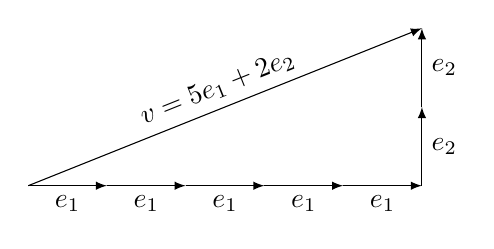
\begin{tikzpicture}[
	point/.style={circle,draw,very thin,fill,inner sep=0pt,minimum size=4pt},
	vector/.style={-latex},
]
	\draw[vector] (0,0) to node[above,sloped] {$\uvec{v} = 5\uvec{e}_1 + 2\uvec{e}_2$} (5,2);
	\foreach \x in {0,1,...,4} {
		\draw[vector] (\x,0) to node[below] {$\uvec{e}_1$} (\x+1,0);
	}
	\foreach \y in {0,1} {
		\draw[vector] (5,\y) to node[right] {$\uvec{e}_2$} (5,\y+1);
	}
\end{tikzpicture}
